

\thispagestyle{empty}\cleardoublepage
\addcontentsline{toc}{section}{Session A: Musical objects}
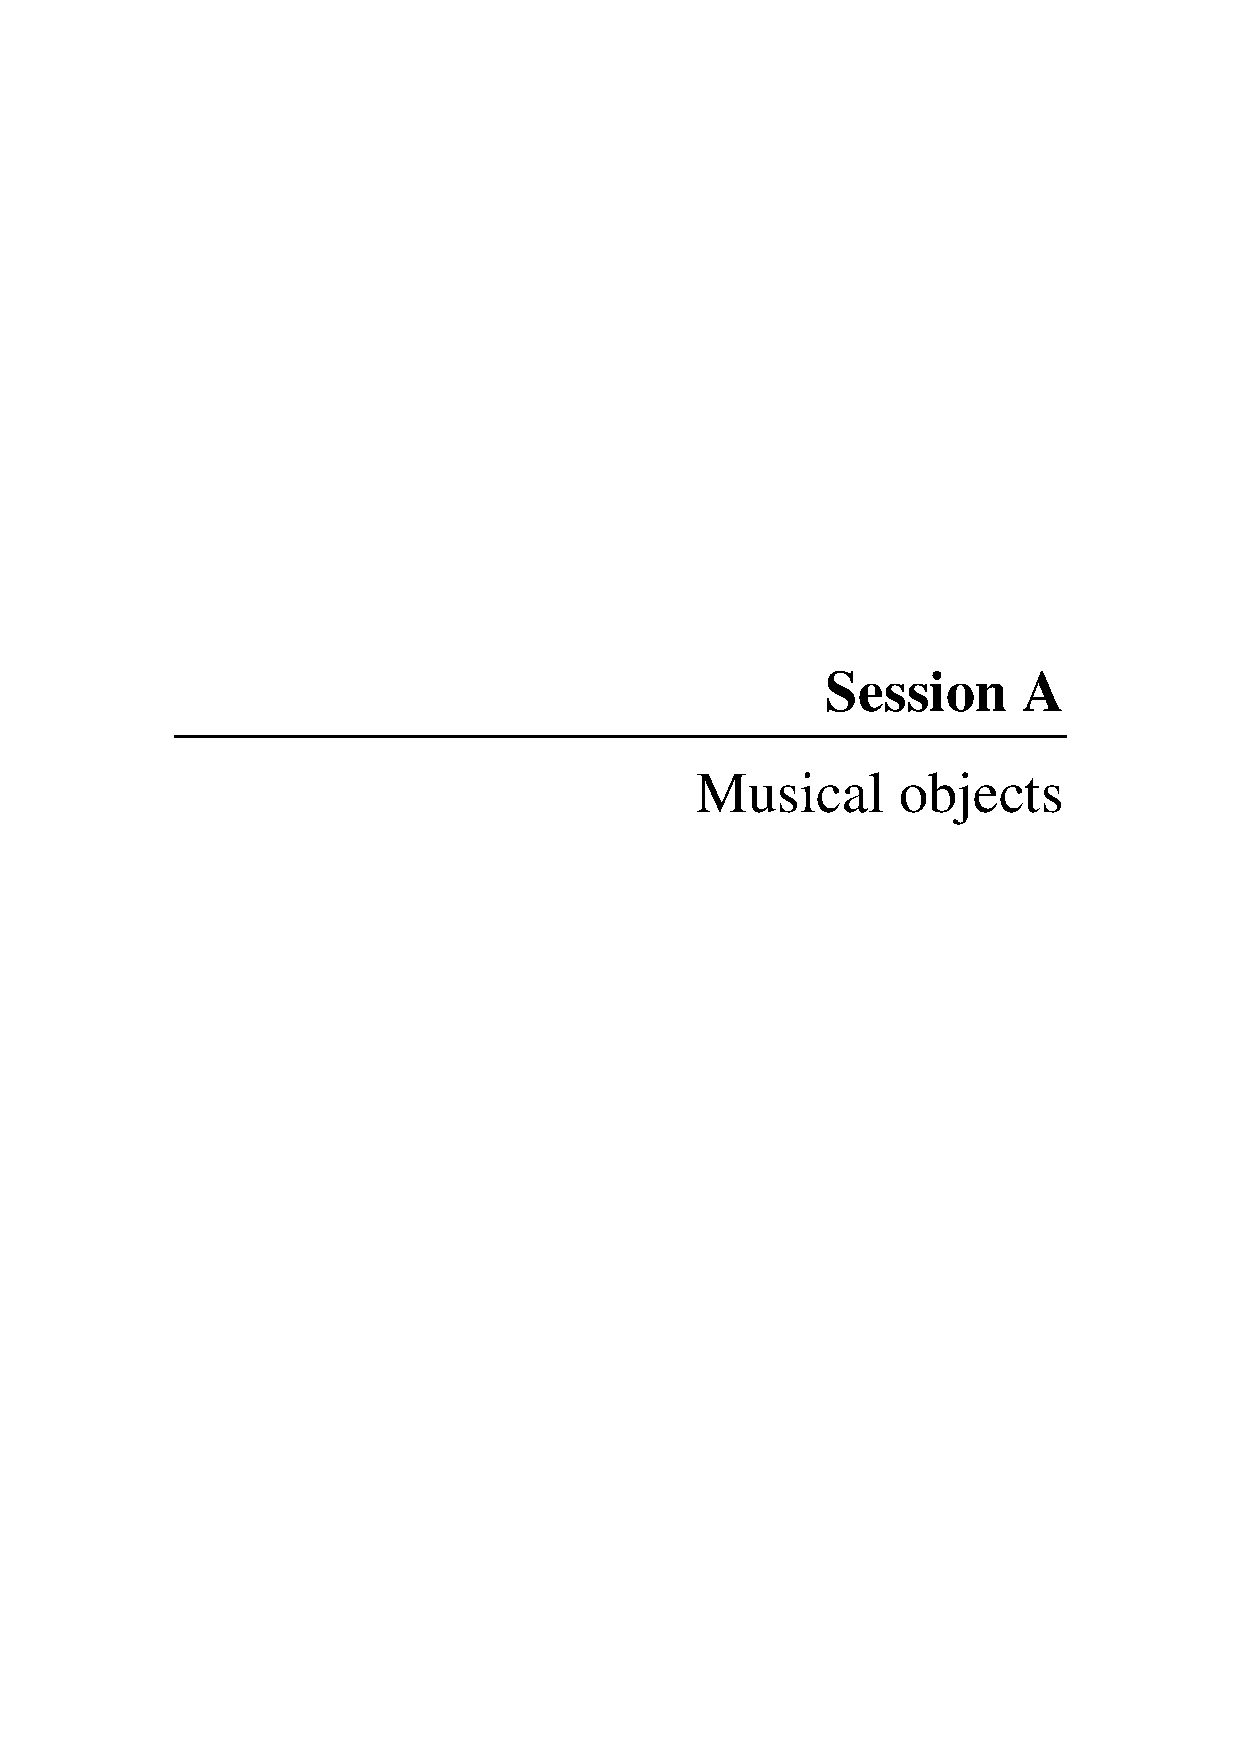
\includepdf[pages=1,pagecommand=\thispagestyle{empty}]{external/12_Sessions.pdf}%
\thispagestyle{empty}\cleardoublepage

\includepaper{A Confidence Measure For Key Labelling}{Roman B. Gebhardt, Michael Stein, Athanasios Lykartsis}{articles/72_Paper}
\includepaper{Improved Chord Recognition by Combining Duration and Harmonic Language Models}{Filip Korzeniowski, Gerhard Widmer}{articles/300_Paper}
\includepaper{Using musical relationships between chord labels in Automatic Chord Extraction tasks}{Tristan Carsault, Jerome Nika, Philippe Esling}{articles/231_Paper}
\includepaper{A Predictive Model for Music based on Learned Interval Representations}{Stefan Lattner, Maarten Grachten, Gerhard Widmer}{articles/179_Paper}
\includepaper{An End-to-end Framework for Audio-to-Score Music Transcription on Monophonic Excerpts}{Miguel A. Román, Antonio Pertusa, Jorge Calvo-Zaragoza}{articles/87_Paper}
\includepaper{Evaluating Automatic Polyphonic Music Transcription}{Andrew McLeod, Mark Steedman}{articles/148_Paper}
\includepaper{Onsets and Frames: Dual-Objective Piano Transcription}{Curtis Hawthorne, Erich Elsen, Jialin Song, Adam Roberts, Ian Simon, Colin Raffel, Jesse Engel, Sageev Oore, Douglas Eck}{articles/19_Paper}
\includepaper{Player Vs Transcriber: A Game Approach To Data Manipulation For Automatic Drum Transcription}{Carl Southall, Ryan Stables, Jason Hockman}{articles/24_Paper}
\includepaper{A Flexible Approach to Automated Harmonic Analysis: Multiple Annotations of Chorales by Bach and Prætorius}{Nathaniel Condit-Schultz, Yaolong Ju, Ichiro Fujinaga}{articles/283_Paper}
\includepaper{Evaluating a collection of Sound-Tracing Data of Melodic Phrases}{Tejaswinee Kelkar, Udit Roy, Alexander Refsum Jensenius}{articles/209_Paper}
\includepaper{Main Melody Estimation with Source-Filter NMF and CRNN}{Dogac Basaran, Slim Essid, Geoffroy Peeters}{articles/273_Paper}
\includepaper{Functional Harmony Recognition of Symbolic music data with Multi-task Recurrent Neural Networks}{Tsung-Ping Chen, Li Su}{articles/178_Paper}
\includepaper{A single-step approach to musical tempo estimation using a convolutional neural network}{Hendrik Schreiber, Meinard Müller}{articles/141_Paper}
\includepaper{Analysis of Common Design Choices in Deep Learning Systems for Downbeat Tracking}{Magdalena Fuentes, Brian McFee, Hélène C. Crayencour, Slim Essid, Juan Pablo Bello}{articles/203_Paper}
\includepaper{Meter Detection and Alignment of MIDI Performance}{Andrew McLeod, Mark Steedman}{articles/136_Paper}
\includepaper{A Timbre-based Approach to Estimate Key Velocity from Polyphonic Piano Recordings}{Dasaem Jeong, Taegyun Kwon, Juhan Nam}{articles/196_Paper}
\includepaper{Timbre Discrimination for Brief Instrument Sounds}{Francesco Bigoni, Sofia Dahl}{articles/249_Paper}
\includepaper{Frame-level Instrument Recognition by Timbre and Pitch}{Yun-Ning Hung, Yi-Hsuan Yang}{articles/55_Paper}


\thispagestyle{empty}\cleardoublepage
\addcontentsline{toc}{section}{Session B: Generation, visual}
\includepdf[pages=2,pagecommand=\thispagestyle{empty}]{external/12_Sessions.pdf}%
\thispagestyle{empty}\cleardoublepage

\includepaper{Interactive Arrangement of Chords and Melodies Based on a Tree-Structured Generative Model}{Hiroaki Tsushima, Eita Nakamura, Katsutoshi Itoyama, Kazuyoshi Yoshii}{articles/1_Paper}
\includepaper{A Generalized Parsing Framework for Generative Models of Harmonic Syntax}{Daniel Harasim, Martin Rohrmeier, Timothy J. O'Donnell}{articles/258_Paper}
\includepaper{An energy-based generative sequence model for testing sensory theories of Western harmony}{Peter M. C. Harrison, Marcus T. Pearce}{articles/215_Paper}
\includepaper{Automatic, Personalized, and Flexible Playlist Generation using Reinforcement Learning}{Shun-Yao Shih, Heng-Yu Chi}{articles/18_Paper}
\includepaper{Bridging audio analysis, perception and synthesis with perceptually-regularized variational timbre spaces}{Philippe Esling, Axel Chemla--Romeu-Santos, Adrien Bitton}{articles/219_Paper}
\includepaper{Conditioning Deep Generative Raw Audio Models for Structured Automatic Music}{Rachel Manzelli, Vijay Thakkar, Ali Siahkamari, Brian Kulis}{articles/192_Paper}
\includepaper{Convolutional Generative Adversarial Networks with Binary Neurons for Polyphonic Music Generation}{Hao-Wen Dong, Yi-Hsuan Yang}{articles/218_Paper}
\includepaper{Cover Song Synthesis by Analogy}{Christopher Tralie}{articles/103_Paper}
\includepaper{Part-invariant Model for Music Generation and Harmonization}{Yujia Yan, Ethan Lustig, Joseph VanderStel, Zhiyao Duan}{articles/293_Paper}
\includepaper{Evaluating language models of tonal harmony}{David Sears, Filip Korzeniowski, Gerhard Widmer}{articles/262_Paper}
\includepaper{Skeleton plays piano: online generation of pianist body movements from MIDI performance}{Bochen Li, Akira Maezawa, Zhiyao Duan}{articles/109_Paper}
\includepaper{Towards Full-Pipeline Handwritten OMR with Musical Symbol Detection by U-Nets}{Jan Hajič jr., Matthias Dorfer, Gerhard Widmer, Pavel Pecina}{articles/175_Paper}
\includepaper{Searching Page-Images of Early Music Scanned with OMR: A Scalable Solution Using Minimal Absent Words}{Tim Crawford, Golnaz Badkobeh, David Lewis}{articles/210_Paper}
\includepaper{Optical Music Recognition in Mensural Notation with Region-based Convolutional Neural Networks}{Alexander Pacha, Jorge Calvo-Zaragoza}{articles/32_Paper}
\includepaper{Camera-PrIMuS: Neural End-to-End Optical Music Recognition on Realistic Monophonic Scores}{Jorge Calvo-Zaragoza, David Rizo}{articles/33_Paper}
\includepaper{Document Analysis of Music Score Images with Selectional Auto-Encoders}{Francisco Castellanos, Jorge Calvo-Zaragoza, Gabriel Vigliensoni, Ichiro Fujinaga}{articles/93_Paper}
\includepaper{Genre-Agnostic Key Classification With Convolutional Neural Networks}{Filip Korzeniowski, Gerhard Widmer}{articles/7_Paper}
\includepaper{Deep Watershed Detector for Music Object Recognition}{Lukas Tuggener, Ismail Elezi, Jürgen Schmidhuber, Thilo Stadelmann}{articles/225_Paper}


\thispagestyle{empty}\cleardoublepage
\addcontentsline{toc}{section}{Session C: Source separation, symbolic, emotion}
\includepdf[pages=3,pagecommand=\thispagestyle{empty}]{external/12_Sessions.pdf}%
\thispagestyle{empty}\cleardoublepage

\includepaper{Deep neural networks with voice entry estimation heuristics for voice separation in symbolic music representations}{Reinier de Valk, Tillman Weyde}{articles/304_Paper}
\includepaper{Music Source Separation Using Stacked Hourglass Networks}{Sungheon Park, Taehoon Kim, Kyogu Lee, Nojun Kwak}{articles/138_Paper}
\includepaper{The Northwestern University Source Separation Library}{Ethan Manilow, Prem Seetharaman, Bryan Pardo}{articles/37_Paper}
\includepaper{Improving Bass Saliency Estimation using Transfer Learning and Label Propagation}{Jakob Abeßer, Stefan Balke, Meinard Müller}{articles/143_Paper}
\includepaper{Improving Peak-picking Using Multiple Time-step Loss Functions}{Carl Southall, Ryan Stables, Jason Hockman}{articles/25_Paper}
\includepaper{Zero-Mean Convolutions for Level-Invariant Singing Voice Detection}{Jan Schlüter, Bernhard Lehner}{articles/189_Paper}
\includepaper{Music Generation and Transformation with Moment Matching-Scattering Inverse Networks}{Mathieu Andreux, Stéphane Mallat}{articles/131_Paper}
\includepaper{Wave-U-Net: A Multi-Scale Neural Network for End-to-End Audio Source Separation}{Daniel Stoller, Sebastian Ewert, Simon Dixon}{articles/205_Paper}
\includepaper{SE and SNL diagrams: Flexible data structures for MIR}{Melissa R. McGuirl, Katherine M. Kinnaird, Claire Savard, Erin H. Bugbee}{articles/105_Paper}
\includepaper{JSYMBOLIC 2.2: Extracting Features from Symbolic Music for use in Musicological and MIR Research}{Cory McKay, Julie Cumming, Ichiro Fujinaga}{articles/26_Paper}
\includepaper{Relevance of musical features for cadence detection}{Louis Bigo, Laurent Feisthauer, Mathieu Giraud, Florence Levé}{articles/243_Paper}
\includepaper{On the Relationships between Music-induced Emotion and Physiological Signals}{Xiao Hu, Fanjie Li, Jeremy T. D. Ng}{articles/115_Paper}
\includepaper{Music Mood Detection Based on Audio and Lyrics with Deep Neural Net}{Rémi Delbouys, Romain Hennequin, Francesco Piccoli, Jimena Royo-Letelier, Manuel Moussallam}{articles/99_Paper}
\includepaper{Identifying Emotions in Opera Singing: Implications of Adverse Acoustic Conditions}{Emilia Parada-Cabaleiro, Maximilian Schmitt, Anton Batliner, Simone Hantke, Giovanni Costantini, Klaus Scherer, Bjoern Schuller}{articles/22_Paper}
\includepaper{Musical Texture and Expressivity Features for Music Emotion Recognition}{Renato Panda, Ricardo Malheiro, Rui Pedro Paiva}{articles/250_Paper}
\includepaper{Shared generative representation of auditory concepts and EEG to reconstruct perceived and imagined music}{André Ofner, Sebastian Stober}{articles/101_Paper}
\includepaper{Exploring Musical Relations Using Association Rule Networks}{Renan de Padua, Verônica Oliveira de Carvalho, Solange Rezende, Diego Furtado Silva}{articles/268_Paper}


\thispagestyle{empty}\cleardoublepage
\addcontentsline{toc}{section}{Session D: Corpora and voice}
\includepdf[pages=4,pagecommand=\thispagestyle{empty}]{external/12_Sessions.pdf}%
\thispagestyle{empty}\cleardoublepage

\includepaper{A Crowdsourced Experiment for Tempo Estimation of Electronic Dance Music}{Hendrik Schreiber, Meinard Müller}{articles/220_Paper}
\includepaper{Computational Corpus Analysis: A Case Study on Jazz Solos}{Christof Weiss, Stefan Balke, Jakob Abesser, Meinard Müller}{articles/23_Paper}
\includepaper{Controlled Vocabularies for Music Metadata}{Pasquale Lisena, Konstantin Todorov, Cécile Cecconi, Françoise Leresche, Isabelle Canno, Frédéric Puyrenier, Martine Voisin, Thierry Le Meur, Raphaël Troncy}{articles/68_Paper}
\includepaper{DALI: a large Dataset of synchronized Audio, LyrIcs and notes, automatically created using teacher-student machine learning paradigm.}{Gabriel Meseguer-Brocal, Alice Cohen-Hadria, Geoffroy Peeters}{articles/35_Paper}
\includepaper{OpenMIC-2018: An open data-set for multiple instrument recognition}{Eric Humphrey, Simon Durand, Brian McFee}{articles/248_Paper}
\includepaper{From Labeled to Unlabeled Data – On the Data Challenge in Automatic Drum Transcription}{Chih-Wei Wu, Alexander Lerch}{articles/185_Paper}
\includepaper{GuitarSet: A Dataset for Guitar Transcription}{Qingyang Xi, Rachel Bittner, Johan Pauwels, Xuzhou Ye, Juan Pablo Bello}{articles/188_Paper}
\includepaper{Musical-Linguistic Annotations of Il Lauro Secco}{Emilia Parada-Cabaleiro, Maximilian Schmitt, Anton Batliner, Bjoern Schuller}{articles/11_Paper}
\includepaper{VocalSet: A Singing Voice Dataset}{Julia Wilkins, Prem Seetharaman, Alison Wahl, Bryan Pardo}{articles/114_Paper}
\includepaper{The NES Music Database: A multi-instrumental dataset with expressive performance attributes}{Chris Donahue, Huanru Henry Mao, Julian McAuley}{articles/265_Paper}
\includepaper{Audio-Aligned Jazz Harmony Dataset for Automatic Chord Transcription and Corpus-based Research}{Vsevolod Eremenko, Emir Demirel, Baris Bozkurt, Xavier Serra}{articles/206_Paper}
\includepaper{Methodologies for Creating Symbolic Corpora of Western Music Before 1600}{Julie Cumming, Cory McKay, Jonathan Stuchbery, Ichiro Fujinaga}{articles/46_Paper}
\includepaper{Precision of Sung Notes in Carnatic Music}{Venkata Viraraghavan, Rangarajan Aravind, Hema Murthy}{articles/120_Paper}
\includepaper{Revisiting Singing Voice Detection: A quantitative review and the future outlook}{Kyungyun Lee, Keunwoo Choi, Juhan Nam}{articles/38_Paper}
\includepaper{Vocals in Music Matter: the Relevance of Vocals in the Minds of Listeners}{Andrew Demetriou, Andreas Jansson, Aparna Kumar, Rachel Bittner}{articles/98_Paper}
\includepaper{Vocal melody extraction with semantic segmentation and audio-symbolic domain transfer learning}{Wei Tsung Lu, Li Su}{articles/286_Paper}
\includepaper{Empirically Weighting the Importance of Decision Factors for Singing Preference}{Michael Barone, Karim Ibrahim, Chitralekha Gupta, Ye Wang}{articles/117_Paper}


\thispagestyle{empty}\cleardoublepage
\addcontentsline{toc}{section}{Session E: Timbre, tagging, similarity, patterns and alignment}
\includepdf[pages=5,pagecommand=\thispagestyle{empty}]{external/12_Sessions.pdf}%
\thispagestyle{empty}\cleardoublepage

\includepaper{Analysis by classification: A comparative study of annotated and algorithmically extracted patterns in symbolic music data}{Iris Yuping Ren, Anja Volk, Wouter Swierstra, Remco Veltkamp}{articles/75_Paper}
\includepaper{Generalized Skipgrams for Pattern Discovery in Polyphonic Streams}{Christoph Finkensiep, Markus Neuwirth, Martin Rohrmeier}{articles/202_Paper}
\includepaper{Comparison of Audio Features for Recognition of Western and Ethnic Instruments in Polyphonic Mixtures}{Igor Vatolkin, Günter Rudolph}{articles/139_Paper}
\includepaper{Instrudive: A Music Visualization System Based on Automatically Recognized Instrumentation}{Takumi Takahashi, Satoru Fukayama, Masataka Goto}{articles/63_Paper}
\includepaper{Instrument Activity Detection in Polyphonic Music using Deep Neural Networks}{Siddharth Gururani, Cameron Summers, Alexander Lerch}{articles/275_Paper}
\includepaper{Jazz Solo Instrument Classification with Convolutional Neural Networks, Source Separation, and Transfer Learning}{Juan S. Gómez, Jakob Abeßer, Estefanía Cano}{articles/145_Paper}
\includepaper{Aligned sub-Hierarchies: a structure-based approach to the cover song task}{Katherine M. Kinnaird}{articles/81_Paper}
\includepaper{Audio-to-Score Alignment using Transposition-invariant Features}{Andreas Arzt, Stefan Lattner}{articles/166_Paper}
\includepaper{Semi-supervised lyrics and solo-singing alignment}{Chitralekha Gupta, Rong Tong, Haizhou Li, Ye Wang}{articles/30_Paper}
\includepaper{Concert Stitch: Organization and Synchronization of Crowd Sourced Recordings}{Vinod Subramanian, Alexander Lerch}{articles/182_Paper}
\includepaper{A data-driven approach to mid-level perceptual musical feature modeling}{Anna Aljanaki, Mohammad Soleymani}{articles/183_Paper}
\includepaper{Disambiguating Music Artists at Scale with Audio Metric Learning}{Jimena Royo-Letelier, Romain Hennequin, Viet-Anh Tran, Manuel Moussallam}{articles/211_Paper}
\includepaper{Driftin' down the scale: Dynamic time warping in the presence of pitch drift and transpositions}{Simon Waloschek, Aristotelis Hadjakos}{articles/97_Paper}
\includepaper{End-to-end Learning for Music Audio Tagging at Scale}{Jordi Pons, Oriol Nieto, Matthew Prockup, Erik M. Schmidt, Andreas F. Ehmann, Xavier Serra}{articles/191_Paper}
\includepaper{Audio based disambiguation of music genre tags}{Romain Hennequin, Jimena Royo-Letelier, Manuel Moussallam}{articles/163_Paper}
\includepaper{Learning Domain-Adaptive Latent Representations of Music Signals Using Variational Autoencoders}{Yin-Jyun Luo, Li Su}{articles/169_Paper}
\includepaper{Learning Interval Representations from Polyphonic Music Sequences}{Stefan Lattner, Maarten Grachten, Gerhard Widmer}{articles/172_Paper}


\thispagestyle{empty}\cleardoublepage
\addcontentsline{toc}{section}{Session F: Machine and human learning of music}
\includepdf[pages=6,pagecommand=\thispagestyle{empty}]{external/12_Sessions.pdf}%
\thispagestyle{empty}\cleardoublepage

\includepaper{Influences on the Social Practices Surrounding Commercial Music Services: A Model for Rich Interactions}{Louis Spinelli, Josephine Lau, Liz Pritchard, Jin Ha Lee}{articles/52_Paper}
\includepaper{Investigating Cross-Country Relationship between Users' Social Ties and Music Mainstreaminess}{Christine Bauer, Markus Schedl}{articles/130_Paper}
\includepaper{Listener Anonymizer: Camouflaging Play Logs to Preserve User's Demographic Anonymity}{Kosetsu Tsukuda, Satoru Fukayama, Masataka Goto}{articles/78_Paper}
\includepaper{On the Impact of Music on Decision Making in Cooperative Tasks}{Elad Liebman, Corey N. White, Peter Stone}{articles/298_Paper}
\includepaper{VenueRank: Identifying Venues that Contribute to Artist Popularity}{Emmanouil Krasanakis, Emmanouil Schinas, Symeon Papadopoulos, Yiannis Kompatsiaris, Pericles Mitkas}{articles/91_Paper}
\includepaper{The Many Faces of Users: Modeling Musical Preference}{Eva Zangerle, Martin Pichl}{articles/128_Paper}
\includepaper{Representation Learning of Music Using Artist Labels}{Jiyoung Park, Jongpil Lee, Jangyeon Park, Jung-Woo Ha, Juhan Nam}{articles/168_Paper}
\includepaper{StructureNet: Inducing Structure in Generated Melodies}{Gabriele Medeot, Srikanth Cherla, Katerina Kosta, Matt McVicar, Samer Abdallah, Marco Selvi, Ed Newton-Rex, Kevin Webster}{articles/126_Paper}
\includepaper{Summarizing and Comparing Music Data and Its Application on Cover Song Identification}{Diego Furtado Silva, Felipe Falcão, Nazareno Andrade}{articles/36_Paper}
\includepaper{Transferring the Style of Homophonic Music Using Recurrent Neural Networks and Autoregressive Model}{Wei Tsung Lu, Li Su}{articles/107_Paper}
\includepaper{MIDI-VAE: Modeling Dynamics and Instrumentation of Music with Applications to Style Transfer}{Gino Brunner, Andres Konrad, Yuyi Wang, Roger Wattenhofer}{articles/204_Paper}
\includepaper{Understanding a Deep Machine Listening Model Through Feature Inversion}{Saumitra Mishra, Bob L. Sturm, Simon Dixon}{articles/272_Paper}
\includepaper{Comparing RNN Parameters for Melodic Similarity}{Tian Cheng, Satoru Fukayama, Masataka Goto}{articles/61_Paper}
\includepaper{Visualization of audio data using stacked graphs}{Mathieu Lagrange, Mathias Rossignol, Grégoire Lafay}{articles/96_Paper}
\includepaper{Two web applications for exploring melodic patterns in jazz solos}{Klaus Frieler, Frank Höger, Martin Pfleiderer, Simon Dixon}{articles/177_Paper}
\includepaper{Learning to Listen, Read, and Follow: Score Following as a Reinforcement Learning Game}{Matthias Dorfer, Florian Henkel, Gerhard Widmer}{articles/45_Paper}
\includepaper{Matrix Co-Factorization for Cold-Start Recommendation}{Olivier Gouvert, Thomas Oberlin, Cédric Févotte}{articles/142_Paper}
